
Replay attacks are an example of low-effort spoofing; they require simply the replaying of a previously captured speech signal.  
In the absence of suitable countermeasures and considering the widespread availability of consumer devices with reasonable quality sound systems, replay attacks can typically be realised with ease.  
%The risk of playback attacks is even higher if recordings of a speaker are publicly available and is
Furthermore, they are pertinent in the case of both text-dependent and text-independent systems through the cutting and pasting of short speech intervals.  
Paradoxically, given that they have potential to attenuate channel effects which might be introduced through recording and replaying, channel-compensation and other techniques which aim to attenuate intersession variability have potential to work in favour of the replay attacker.
Since almost all state-of-the-art speaker verification systems include some form of intersession compensation, then one must consider most systems at least somewhat vulnerable. 
All of these factors point towards the significant threat of replay attacks and the importance of developing suitable anti-spoofing countermeasures.

This section... describe briefly the contents of the section.

% COMMENT: note that I removd the following.  I don't find that is really necessary for the other material in this section and it will help to differentiate more from the BIOSIG paper if we move this material to the section which relates to your contribution rather than the past work.

%When modelling a replay attack one should take into account the impact of the following elements:

%\begin{itemize}
%\item acoustic effects introduced by the recording device;
%\item acoustic conditions in the environment where the voice was acquired;
%\item acoustic effects of the replay device, and the
%\item acoustic conditions in the environment where the attack takes place. 
%\end{itemize}

%\begin{figure}
%	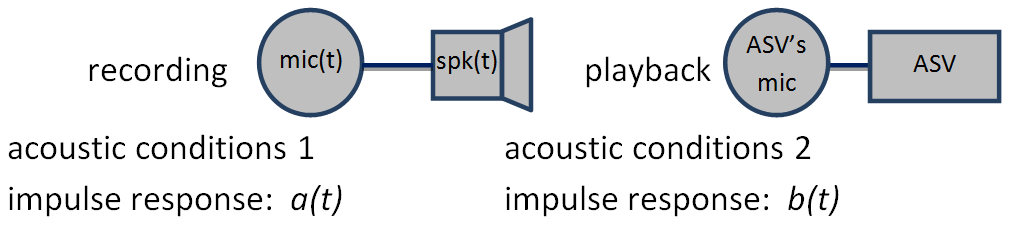
\includegraphics[width=1\linewidth]{Figs/replay.png}
%
%	\caption{Schematic diagram of replay.}
%	\label{fig::Replay}
%\end{figure}


\begin{figure*}
	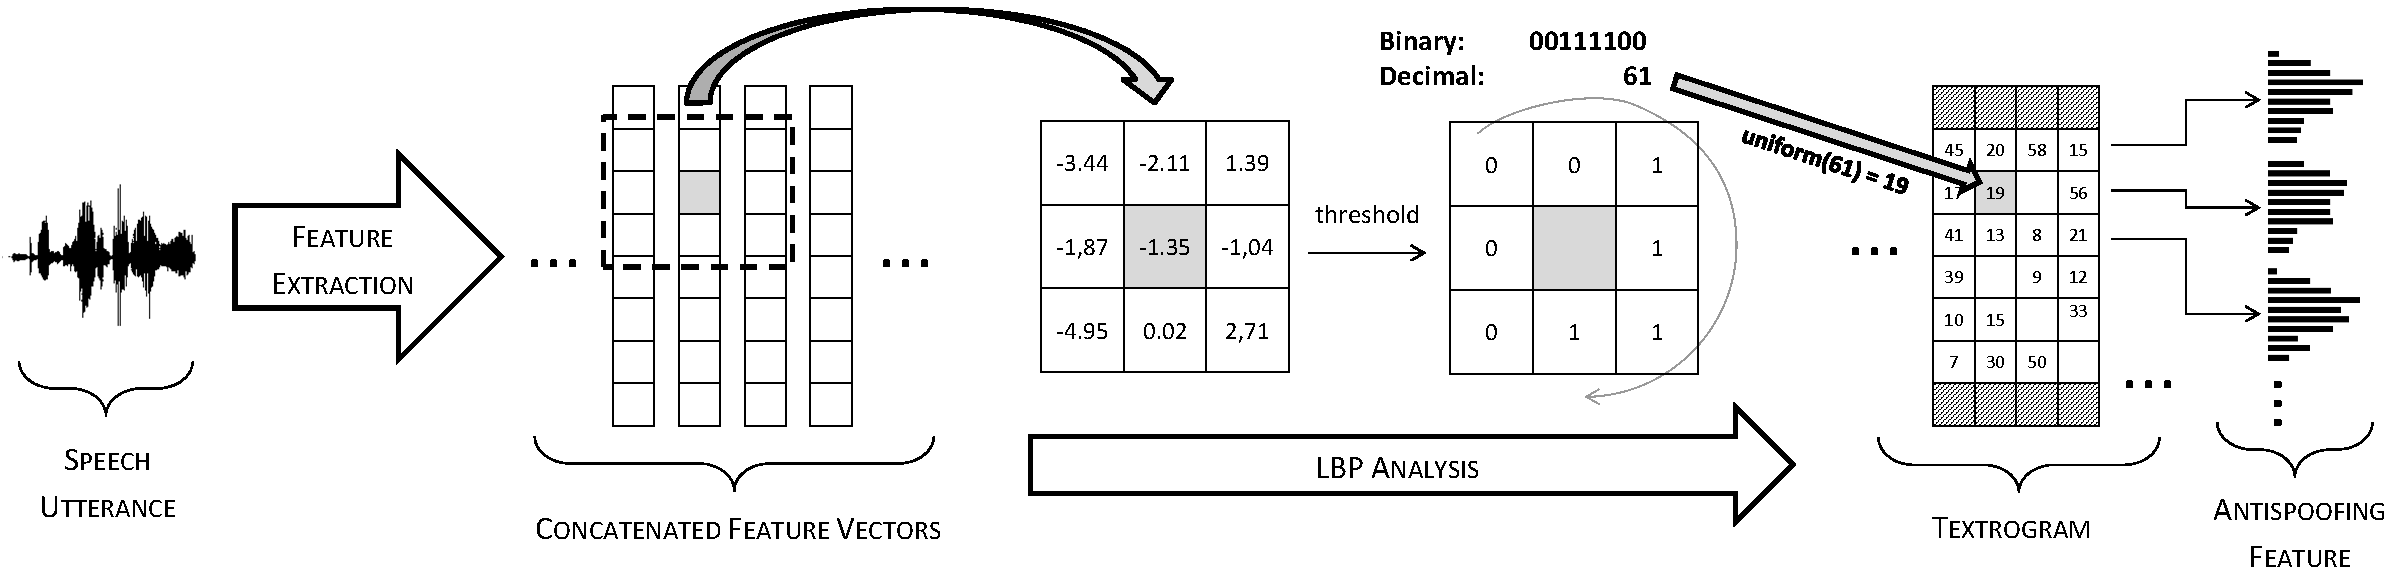
\includegraphics[width=1\linewidth]{Figs/LBPfeature.pdf}

	\caption{Schematic diagram of forming a feature vector in the LBP-based countermeasure.}
	\label{fig:LBPfeature}
\end{figure*}



%If $x(t)$ is the speech signal of the client, the playback (spoofing) signal $y(t)$ can be represented by:

%\begin{equation}
%y(t) = x(t)* mic(t) * a(t) * spk(t) * b(t)
%\label{eq::playback}
%\end{equation}

%where * denotes convolution, $mic(t)$ and $spk(t)$ are impulse responses of the microphone and the speaker, respectively, and $a(t)$ and $b(t)$ are impulse responses of recording and replay environments, respectively (see Fig.~\ref{fig::Replay}). 


\begin{table*}
%\ninept
\begin{center}
    \begin{tabular}{ l | c c c c }
    \hline
     	 Attack & Na\"{i}ve impostor &  Replay & Voice conversion & Speech synthesis\\ 
    \hline
  Speech used & \begin{tabular}{ c } impostor's\\(genuine) \end{tabular} & client's &  \begin{tabular}{ c } impostor's\\(converted) \end{tabular} & synthetic\\
Effort & zero & low & medium-high & high\\
Effectiveness & low &  \textbf{(?)} & medium-high & high\\
 \hline
\hline
    \end{tabular}
    \caption{Comparison of four different attacks in terms of speech used,  required effort and effectiveness.}
		\label{tab::attacks}
   \end{center}
\end{table*}


%\subsection{Research on replay spoofing and replay countermeasures}
\subsection{Previous work}

{\bfseries COMMENT: It doesn't seem right to have so little text on the threat when there is so much on countermeasues.}
While a great deal of attention has been paid to medium- and high-effort spoofing attacks (reviews can be found in~\cite{handbookChapter,specComJournal}), only few studies have addressed replay.  
The work in~\cite{Lindberg1999} assessed the vulnerabilities of an HMM-based, text-dependent ASV system with concatenated digits.  
While results showed that replay attacks are highly effective, experiments were conducted with data collected from only two speakers.
The work in~\cite{Villalba2010} investigated replay using recordings which were collected with close-talk or far-field microphones and then replayed over an analogue or digital telephony channel. 
The work was conducted with a similarly small corpus with five speakers and showed that a joint factor analysis (JFA) ASV system was vulnerable to replay attacks -- the FAR at the EER threshold increased from 1\% to almost 70\%. 


{\bfseries COMMENT: you don't have any references for challenge-response?}
Given that only little work has investigated attacks, it is not surprising that the work in anti-spoofing is similarly limited.  
One obvious approach involves challenge-response systems which require the speaker to utter a prompted ad hoc phrase~\cite{???}. 
Challenge-response mechanisms are a form of passive countermeasure; more active countermeasures have also been proposed.
One approach involves the storing of previous access attempts and their comparison to new attempts~\cite{Shang2010}. 
The detection of high similarity was shown to serve as an effective means of identifying replay attack, albeit in a rather constrained scenario.
%The experiments showed that this method caused a decrease in EER in  most of the cases, however, this method is useless if there were no previous access trials with a given recording. 

Other methods 
%work in investigated the use of channel noise statistics as a means of detecting replay attacks.  These methods 
essentially aim to detect the presence of an unexpected channel, i.e. channel artefacts indicative of recording and replaying.
Two such algorithms were reported in~\cite{Wang2011} and show reductions in 
% The authors proposed two variants of their countermeasure, and they managed to decrease the EER from
an equal error rate (EER) from 40\% to 10\% with a baseline GMM-UBM system subjected to replay attacks.
Villalba and Lleida~\cite{Villalba2011} investigated a similar, channel-detection approach.  
Since many logical and physical access based ASV systems can reasonably expect close-talk speech, and since some recordings will be made surreptitiously or at-distance, the detection of far-field speech serves as an effective countermeasure.  
Villalba and Lleida's work showed that far-field recordings cause changes in the speech signal envelope, changes which can be easily detected with 90\% recognition accuracy.
% ; therefore they extracted 12 parameters describing the envelope and, based on them, trained a binary SVM classifier in order to discriminate far-field speech from close-talk speech. The authors claimed that they reached the far-field recognition rate of more than 90\%.


\subsection{A countermeasure based on local binary patterns}

{\bfseries COMMENT: Probably not a great idea to write so much about this one technique (our own) whereas you allocate only a very small amount of text to other work (by other authors).  I suggest to greatly reduce and to merge with the material above in one section on previous work.}

Local binary patterns (LBP) technique is a countermeasure which we previously proposed in~\cite{Alegre2013a} against attacks using voice conversion, speech synthesis and artificial signals. It is based on the hypothesis that modifications made through spoofing disturb the natural 'texture' of genuine speech. This technique was adopted from a standard texture analysis approach, known in image processing~\cite{Ojala2002}, to a 2-dimensional 'image' of a speech utterance, where here the image is a mel-scaled cepstrogram appended with dynamic features.

The standard LBP operator is a non-parametric 3x3 kernel which assigns a binary code to each pixel in an image according to the comparison of its intensity value to that of its eight surrounding pixels~\cite{Ojala2002}. This procedure is illustrated in Figure~\ref{fig:LBPfeature}.  A binary value of '1' is assigned when the intensity of neighbouring pixels (here feature components) is higher, whereas a value of '0' is assigned when neighbouring pixels are of lower or equal intensity. Each pixel is thus assigned one of $2^8=256$ binary patterns.

LBPs are determined for each pixel in the mel-scaled cepstrogram thus resulting in a new matrix of reduced dynamic range, here referred to as a 'textrogram'.  The textrogram captures short-time feature motion beyond that in conventional dynamic parametrisation.  The LBP-based countermeasure is based on concatenated histograms formed from the pixel values across each row in the textrogram.  The histograms are individually normalised and their resulting bin values are stacked vertically to obtain a new vector in the same manner as GMM mean-vectors are stacked to form supervectors.  

In~\cite{Alegre2013a} we showed that a LBP-based countermeasure was highly effective for artificial signals, yielding 0\% EER for the five tested ASVs, very effective for speech synthesis attacks (EER values below 1\%) and quite effective for voice conversion -- EERs less than 7\%. Considering the fact that the LBP-based countermeasure hardly relies on prior knowledge on the attack, in this work we decided to try to use it also as a countermeasure against replay attacks.





\subsection{Replay vs. other spoofing attacks}
\label{sec::algorithms::playback}


Table~\ref{tab::attacks} contrasts na\"{i}ve (zero-effort) impostor accesses and spoofing attacks, including replay, voice conversion and speech synthesis.  
They are ordered in terms of the effort or skill needed to implement each attack successfully. 
Replay attacks require slightly increased effort compared to na\"{i}ve imposture (need for recording and replay hardware). 
Voice conversion and speech synthesis require specialised algorithms, in addition to recording hardware to collect, analyse and parameterise the target voice. 
They belong to a class of higher-effort spoofing attacks. 
While voice conversion is still based upon the conversion of an original speech signal, speech synthesis starts with text input. 
Its conversion to a convincing speech signal indicative of a particular speaker requires the most effort of all three attacks.
One may reasonably suppose that the effectiveness of each attack is linked to the effort involved; the higher the effort, the greater the impact on ASV performance. 
However, the results of preliminary experiments described in~\cite{Alegre2014a} found the contrary, showing that replay attacks pose high risk, being effective in overcoming an ASV system while being the easiest to implement.
%can be theis in fact very high, taking into account low-effort required to undertake the attack. This observation will be further verified in this work.

{\bfseries COMMENT:  I would restructure this section.  Having learned that we ought to be concentrating on replay, the subsections on voice conversion and synthesis seem misplaced.  Better to have a general section on spoofing, to introduce replay, voice conversion and speech synthesis and then the comparison.}

\subsubsection{Voice conversion}
\label{ssec:vconv}

When comparing the replay threat with that of voice conversion, we used the approach to voice conversion originally presented in~\cite{Matrouf2005}. At the frame level, the speech signal of a spoofer denoted by $y(t)$ is filtered in the spectral domain as follows:

\begin{equation}
Y'(f) = \frac{\left|H_{x}(f)\right|}{\left|H_{y}(f)\right|}Y(f)
\label{eq:conversioneq}
\end{equation}

\noindent where $H_{x}(f)$ and $H_{y}(f)$ are the vocal tract transfer functions of the targeted speaker and the spoofer respectively.  $Y(f)$ is the spoofer's speech signal whereas $Y'(f)$ denotes the result after voice conversion.  As such, $y(t)$ is mapped or converted towards the target in a spectral-envelope sense, which is sufficient to overcome most ASV systems. 

$H_x(f)$ is determined from a set of two Gaussian mixture models (GMMs).  The first, denoted as the automatic speaker recognition (asr) model in the original work, is related to ASV feature space and utilised for the calculation of a posteriori probabilities whereas the second, denoted as the filtering (fil) model, is a tied model of linear predictive cepstral coding (LPCC) coefficients from which $H_x(f)$ is derived.  LPCC filter parameters are obtained according to:

\begin{equation}
x_{fil} = \sum\limits_{i=1}^{M}p(g_{asr}^{i}|y_{asr}) \mu_{fil}^{i}
\label{eq:EMit}
\end{equation}

\noindent where $p(g_{asr}^{i}|y_{asr})$ is the a posteriori probability of Gaussian component $g_{asr}^{i}$ given the frame $y_{asr}$ and $\mu_{fil}^{i}$ is the mean of component $g_{fil}^{i}$ which is tied to $g_{asr}^{i}$.  $H_{x}(f)$ is estimated from $x_{fil}$ using an LPCC-to-LPC transformation and a time-domain signal is synthesised from converted frames with a standard overlap-add technique. Full details can be found in~\cite{Matrouf2005,Bonastre2006,Bonastre2007}.


\subsubsection{Speech synthesis}

There is a large variety of speech synthesis algorithms, such as formant, diphone or unit-selection based synthesis. State-of-the-art text-to-speech systems use either unit-selection or the hidden Markov model-based synthesis (HTS). Whilst the former requires large amounts of speech data, the latter does not, and can therefore much more easily generate speech targeted towards a specific client. 

Accordingly, in this paper we consider spoofing with HTS synthesis, following the approach described in~\cite{Yamagishi2009}, and using the HMM-based Speech Synthesis System (HTS)\footnote{http://hts.sp.nitech.ac.jp/}. Parametrisation includes STRAIGHT (Speech Transformation and Representation using Adaptive Interpolation of weiGHTed spectrum) features, Mel-cepstrum coefficients and the logarithm of the fundamental frequency (log $F_{0}$) with their delta and acceleration coefficients. Acoustic spectral characteristics and duration probabilities are modelled using multispace distribution hidden semi-Markov models (MSD-HSMM)~\cite{Russell1985}.  Speaker dependent  excitation, spectral and duration models are adapted from corresponding independent models according to a speaker adaptation strategy referred to as constrained structural maximum a posteriori linear regression (CSMAPLR)~\cite{Yamagishi2009a}.  Finally, time domain signals are synthesised using a vocoder based on Mel-logarithmic spectrum approximation (MLSA) filters.  They correspond to STRAIGHT Mel-cepstral coefficients and are driven by a mixed excitation signal and waveforms reconstructed using the pitch synchronous overlap add (PSOLA) method.


